\documentclass{article}%
\usepackage[T1]{fontenc}%
\usepackage[utf8]{inputenc}%
\usepackage{lmodern}%
\usepackage{textcomp}%
\usepackage{lastpage}%
\usepackage[head=40pt,margin=0.5in,bottom=0.6in]{geometry}%
\usepackage{graphicx}%
%
\title{\textbf{Semilla, electricidad y agua piden productores agrícolas}}%
\author{DICK TORRES}%
\date{07/10/2018}%
%
\begin{document}%
\normalsize%
\maketitle%
\textbf{URL: }%
http://www.eluniversal.com/economia/22544/semilla{-}electricidad{-}y{-}agua{-}piden{-}productores{-}agricolas\newline%
%
\textbf{Periodico: }%
EU, %
ID: %
22544, %
Seccion: %
economia\newline%
%
\textbf{Palabras Claves: }%
NO\_TIENE\newline%
%
\textbf{Derecho: }%
3.1, %
Otros Derechos: %
, %
Sub Derechos: %
3.1.1\newline%
%
\textbf{EP: }%
NO\newline%
\newline%
%
\textbf{\textit{Este año la producción de arroz alcanzó el 30\% de la meta esperada, dijo el diputado Luis Silva.}}%
\newline%
\newline%
%
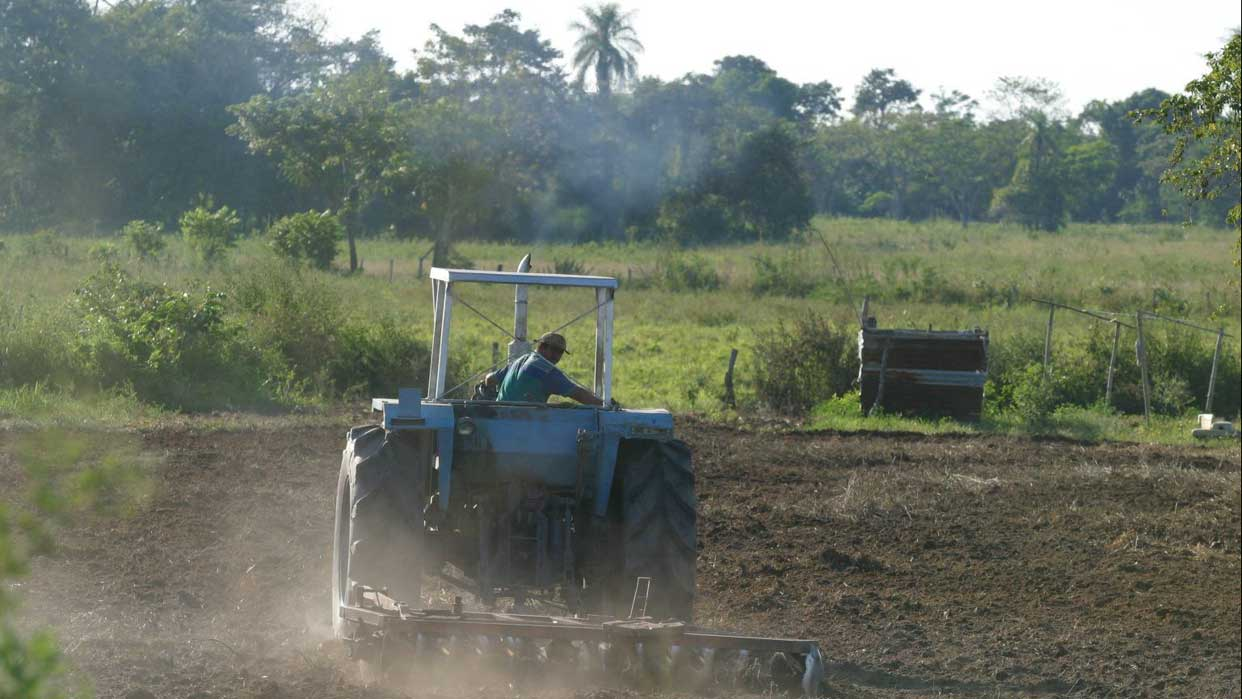
\includegraphics[width=300px]{83.jpg}%
\newline%
%
Caracas.{-} En un 97\% de la superficie agrícola requiere de semilla con calidad genética para aumentar la producción de alimentos en el país.%
\newline%
%
Frente a esa deficiencia el agricultor venezolano tiene que decidir entre dos opciones: No sembrar, en cuyo caso la escasez de alimentos se incrementa en el país; o por el contrario  opta por utilizar semillas extraídas de sus propios cultivos anteriores.%
\newline%
%
La observación es del diputado Luis Silva, presidente Subcomisión Desarrollo Industrial, Comercio y Turismo, de la Asamblea Nacional (AN), quien considera que la productividad agrícola en Venezuela se ha visto afectada, entre otros factores por la escasez de insumo, pero fundamentalmente por la falta de semillas certificadas y con calidad genética para lograr un gran rendimiento en todos los rubros; hortaliza, pasto o leguminosas.%
\newline%
%
Indicó que esta segunda alternativa conlleva el riesgo de propagar enfermedades en los campos agrícolas por la aparición de maleza (monte) y con el resultado final hacia una drástica  caída en el rendimiento de los cultivos y por tanto hay menos siembra.%
\newline%
%
Explicó que la semilla de calidad genética es producto de un complejo proceso científico y tecnológico.~“Venezuela no ha alcanzado los niveles para tener semilla competitiva, en algunos rubros como maíz, soya o leguminosa, sorgo, caraota”.%
\newline%
%
Dijo que en materia de investigación, en el país se han logrado avances importantes pero comentó que han sido ignorados por las autoridades agrícolas venezolanas “dando preferencia a la dependencia de semillas del exterior”.%
\newline%
%
Afirmó que la superficie cultivada en Venezuela alcanzó este año el 25\%.\newline%
\newline%
“Este año, la producción de maíz alcanzó el 30\% de la meta esperada y la del arroz 40\%. En materia de sorgo, soya, ajonjolí o girasol, que también se utilizan para la producción de alimentos concentrados, también estuvo afectada”.%
\newline%
%
En cuanto al arroz dijo que los productores están extrayendo semillas de sus propios campos, incrementando el riesgo de contaminar de enfermedades otras parcelas, donde es común observar, en estos casos, que la planta florece o la espiga aparece pero sin grano en su interior, lo que se conoce como baneamiento del cultivo.%
\newline%
%
Planificar la agricultura%
\newline%
%
“Todos los años hay que sembrar; no se puede esperar que llegue la época de siembra para sacar la cuenta de los insumos que se requiere. Es con anticipación hacer el  listado”, recomendó Silva, quien es ingeniero agrónomo, especializado en producción animal.%
\newline%
%
“En octubre estaríamos negociando la semilla del maíz que se cultiva en abril o mayo; también la de sorgo, soya, papa esta última bajó a un 30\%. En 2017 fue un 11\% de abastecimiento y en 2018 se calcula que estará por debajo de ese porcentaje, tampoco se está importando el producto ni la semilla, con lo cual se reduce significativamente el consumo de papa en el país”.%
\newline%
%
Silva propone planificar la siembra en base a un cronograma de actividades en el que se debe tener en cuenta financiamiento a los productores agropecuarios, la asistencia técnica necesaria, acompañado por un agresivo plan de sustitución de maquinaria el cual data desde hace más de 25 años.%
\newline%
%
“Se requiere recuperar la infraestructura agrícola que comprende sistema de riego, silos de almacenamientos, mataderos y vialidad agrícola que en la actualidad se encuentra muy deteriorada lo cual impide que los productos lleguen a los mercados y esas dificultades incrementan los precios a nivel del consumidor”.%
\newline%
%
Agregó que el campo también se ha visto afectado por la falta de un adecuado suministro de energía eléctrica, de agua potable y acueductos rurales.\newline%
\newline%
“No hay ningún estado donde el suministro de agua funciones adecuadamente”, dijo.%
\newline%
%
“El estado Bolívar tiene el 80\% del agua en el país pero el 50\% de los hogares carece de agua potable. Hay la tubería, un día llega y luego tarda otros  30 días en volver, imagínese cómo será la situación en el campo”.%
\newline%
%
Adicionalmente al productor agropecuario hay que proporcionales los servicios de salud y educación.\newline%
\newline%
“Además de la recuperación de la recuperación agrícola es también importante que el Estado garantice la seguridad jurídica, y personal de los productores.%
\newline%
%
Se debe respetar la titularidad del campo, además, medidas de seguridad en la lucha contra las invasiones de fincas, secuestros y asesinatos”.%
\newline%
%
dicktorres@gmail.com%
\newline%
%
\end{document}